\begin{mainquestion}{circuit_graph_and_circuit_001}{Loops, Nodes, and Elements Oh My!}
Consider the following circuit diagram:

\begin{center}
    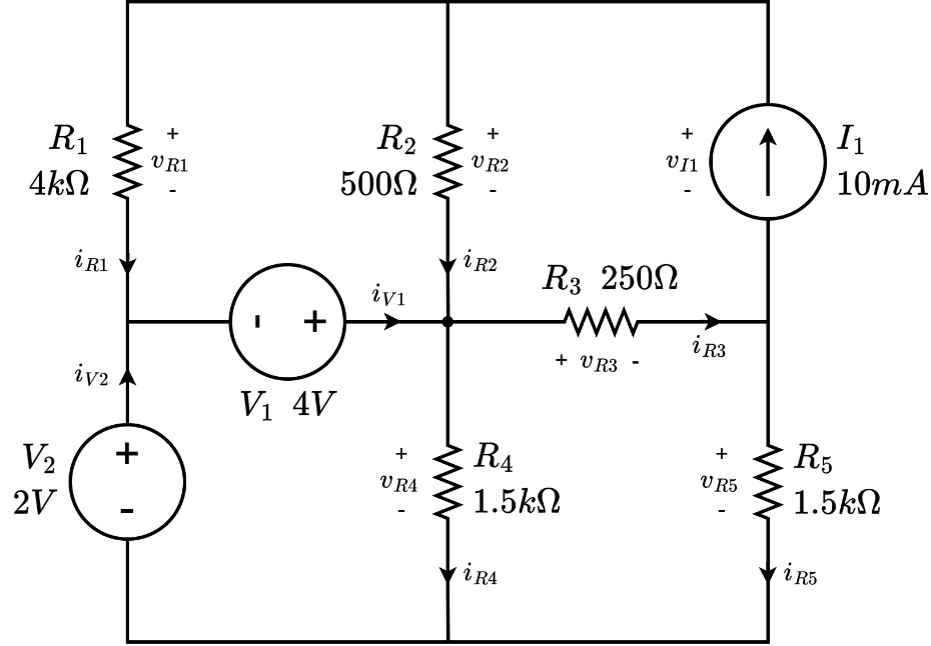
\includegraphics[]{questionbank/networks/circuit_graph/v1/schematic.png}
\end{center}

% =========================================================
\begin{partquestion}{nodes}
{How many nodes are in the circuit?}
\begin{answer}
    There are 5 nodes.
\end{answer}
\end{partquestion}

% =========================================================
\begin{partquestion}{loops}
{How many loops? How many independent loops?}
\begin{answer}
    There are 13 loops, although only 4 of them are independent.
\end{answer}
\end{partquestion}

% =========================================================
\begin{partquestion}{branches}
{How many branches?}
\begin{answer}
    There are 8 branches.  At this point, we can confirm the fundamental theorem of network topology:
    \begin{align*}
        b&=l+n-1\\
        &=4+5-1=8
    \end{align*}
\end{answer}
\end{partquestion}

% =========================================================
\begin{partquestion}{series}
{How many series elements are in the circuit?}
\begin{answer}
    There are no series elements in this circuit:  No two elements share a node exclusively.
\end{answer}
\end{partquestion}

% =========================================================
\begin{partquestion}{parallel}
{How many parallel elements are in the circuit?}
\begin{answer}
    There are no parallel elements in this circuit either!  No two elements share the same node at each of their respective terminals.
\end{answer}
\end{partquestion}
% =========================================================
\begin{partquestion}{unknowns}
{How many unknowns do you have?}
\begin{answer}
There are 7 unknown currents and 6 unknown voltages (don’t forget the voltage across the current source!).
\end{answer}
\end{partquestion}

% =========================================================
\begin{partquestion}{kcl}
{How many KCL equations?}
\begin{answer}
    There are 4 KCL equations (one for all but one node).
\end{answer}
\end{partquestion}

% =========================================================
\begin{partquestion}{kvl}
{How many KVL equations?}
\begin{answer}
There are 4 KVL equations (one for each independent loop).
\end{answer}
\end{partquestion}

% =========================================================
\begin{partquestion}{ohm}
{How many Ohm’s law equations?}
\begin{answer}
There are 5 Ohm’s law equations, one for each resistor.
\end{answer}
\end{partquestion}

% =========================================================
\begin{partquestion}{solve}
{Find all the unknown voltages (in \unit{\volt}) and currents (in \unit{\milli\ampere}) using systematic analysis of all equations found in (\cref{prob:circuit_graph_and_circuit_001:kcl}), (\cref{prob:circuit_graph_and_circuit_001:kvl}), and (\cref{prob:circuit_graph_and_circuit_001:ohm}).}

\begin{answer}

The four KCL equations are (here, current into a node is positive, and current out is negative):

\begin{align}
-i_{R1}-i_{R2}+\qty{10}{\milli\ampere} &= 0 \\
i_{R1}+i_{V2}-i_{V1} &= 0 \\
i_{V1}+i_{R2}-i_{R3}-i_{R4} &= 0 \\
i_{R3}-i_{R5}-\qty{10}{\milli\ampere} &= 0
\end{align}

The four KVL equations are (here the loops were taken in a counterclockwise fashion):

\begin{align}
\qty{4}{\volt}+\qty{2}{\volt}-v_{R4} &= 0 \\
-v_{R5}-v_{R3}+v_{R4} &= 0 \\
-v_{I1}+v_{R2}+v_{R3} &= 0 \\
-v_{R2}+v_{R1}-\qty{4}{\volt} &= 0
\end{align}

The five Ohm's law equations are:

\begin{align}
i_{R1} &= \frac{v_{R1}}{\qty{4}{\kilo\ohm}} \\
i_{R2} &= \frac{v_{R2}}{\qty{0.5}{\kilo\ohm}} \\
i_{R3} &= \frac{v_{R3}}{\qty{0.25}{\kilo\ohm}} \\
i_{R4} &= \frac{v_{R4}}{\qty{1.5}{\kilo\ohm}} \\
i_{R5} &= \frac{v_{R5}}{\qty{1.5}{\kilo\ohm}}
\end{align}

Here is one path to solving the circuit. Starting with (5), it is clear that
$v_{R4}=\qty{6}{\volt}$, and by equation (12)
$i_{R4}=\qty{4}{\milli\ampere}$. Now that $R_4$ is fully solved, equations (4) and (6) form a system of equations between $R_3$ and $R_5$. We substitute (11) and (13) into (4) and substitute $v_{R4}=\qty{6}{\volt}$ into equation (6). This leaves us with the following:
\begin{align*}
\frac{v_{R3}}{\qty{0.25}{\kilo\ohm}}
-
\frac{v_{R5}}{\qty{1.5}{\kilo\ohm}}
&=
\qty{10}{\milli\ampere} \\
v_{R3}+v_{R5}
&=
\qty{6}{\volt}
\end{align*}

Using the method of your choice to solve this system of equations, you will find
\begin{align*}
v_{R3} &= \qty{3}{\volt} \\
v_{R5} &= \qty{3}{\volt}
\end{align*}

Nice! Next use the Ohm's law relations for $R_3$ (11) and $R_5$ (13) to find
$i_{R3}=\qty{12}{\milli\ampere}$ and
$i_{R5}=\qty{2}{\milli\ampere}$.

We can repeat this technique using equations (1) and (8) as well as (9) and (10) to solve the voltages of $R_1$ and $R_2$. Here are the two equations after some massaging:

\begin{align*}
\frac{v_{R1}}{\qty{4}{\kilo\ohm}}
+
\frac{v_{R2}}{\qty{0.5}{\kilo\ohm}}
&=
\qty{10}{\milli\ampere} \\
v_{R1}-v_{R2}
&=
\qty{4}{\volt}
\end{align*}

Again, using the method of your choice to solve this system of equations, you will find

\begin{align*}
v_{R1} &= \qty{8}{\volt} \\
v_{R2} &= \qty{4}{\volt}
\end{align*}

Then plug back into (9) and (10) to find
$i_{R1}=\qty{2}{\milli\ampere}$ and
$i_{R2}=\qty{8}{\milli\ampere}$.

Now that we have all of the resistor branches and currents solved, we should easily be able to find the source unknowns from the remaining equations.

From equation (3) we see that

\[
i_{V1}
=
\qty{12}{\milli\ampere}
-
\qty{4}{\milli\ampere}
=
\qty{8}{\milli\ampere}.
\]

Plugging that into equation (2) reveals

\[
i_{V2}
=
\qty{8}{\milli\ampere}
-
\qty{2}{\milli\ampere}
=
\qty{6}{\milli\ampere}.
\]

Finally, equation (7) can be used to show

\[
v_{I1}
=
\qty{4}{\volt}
+
\qty{3}{\volt}
=
\qty{7}{\volt}.
\]

In summary, the determined values are captured in the tables below:

\begin{table}[htbp]
\centering

\begin{minipage}[t]{0.37\textwidth}
\centering
\begin{tabular}{|l|l|}
\hline
Unknown & Value \\ \hline
$v_{R1}$ & \qty{8}{\volt} \\ \hline
$v_{R2}$ & \qty{4}{\volt} \\ \hline
$v_{R3}$ & \qty{3}{\volt} \\ \hline
$v_{R4}$ & \qty{6}{\volt} \\ \hline
$v_{R5}$ & \qty{3}{\volt} \\ \hline
$v_{I1}$ & \qty{7}{\volt} \\ \hline
$i_{R1}$ & \qty{2}{\milli\ampere} \\ \hline
$i_{R2}$ & \qty{8}{\milli\ampere} \\ \hline
$i_{R3}$ & \qty{12}{\milli\ampere} \\ \hline
$i_{R4}$ & \qty{4}{\milli\ampere} \\ \hline
$i_{R5}$ & \qty{2}{\milli\ampere} \\ \hline
$i_{V1}$ & \qty{8}{\milli\ampere} \\ \hline
$i_{V2}$ & \qty{6}{\milli\ampere} \\ \hline
\end{tabular}
\end{minipage}
\hfill
\begin{minipage}[t]{0.60\textwidth}
\centering
\begin{tabular}{|l|c|c|l|}
\hline
Element & Voltage & Current & Power Flow \\ \hline
$R_1$ & \qty{8}{\volt} & \qty{2}{\milli\ampere} & Absorbing \\ \hline
$R_2$ & \qty{4}{\volt} & \qty{8}{\milli\ampere} & Absorbing \\ \hline
$R_3$ & \qty{3}{\volt} & \qty{12}{\milli\ampere} & Absorbing \\ \hline
$R_4$ & \qty{6}{\volt} & \qty{4}{\milli\ampere} & Absorbing \\ \hline
$R_5$ & \qty{3}{\volt} & \qty{2}{\milli\ampere} & Absorbing \\ \hline
V1 & \qty{4}{\volt} & \qty{8}{\milli\ampere} & Supplying \\ \hline
V2 & \qty{2}{\volt} & \qty{6}{\milli\ampere} & Supplying \\ \hline
I1 & \qty{7}{\volt} & \qty{10}{\milli\ampere} & Supplying \\ \hline
\end{tabular}
\end{minipage}

\end{table}

Note the current reference directions of the ideal sources do not obey the passive sign convention, so if you wanted to use the above table to analyze power you would have to insert negative signs on the currents for the three ideal sources. Adding up the powers for each element, we indeed verify that power is conserved
.
\[
P = 16 + 34 + 36 + 24 + 6 -32 - 12 - 70 = \qty{0}{\watt}
\]

\end{answer}
\end{partquestion}
\end{mainquestion}